\section{Justification}

\subsection*{Detect attacks}
The primary target of the software shall be the detection of potentially malicious IP addresses. By looking at different threat vectors contained within the log files, for example; the frequency of which an IP address accesses the website, or the type of data these access events are attempting to acquire (the log in pages). The software must have the ability to assess and differentiate between similar IP activity (See section on the \nameref{Learning loop and known IPs} for details), an example of the type of attack that could be detected is shown in appendix \ref{Log file example} below.

\subsection*{Analyis of Log files}
Alongside the primary goal of the research application is the ability to analyse website access logs; to address this goal the software needs to be able to read in data. Due to the fact that the data files are not in a easily interpreted format the software should be able to handle the input of varying amounts of data. The data can be represented in a text document, therefore, the software should be able to read a text file quickly and easily. Due to the complexity of the data as explained in this section, the decision was made to allow a flexible amount of data to be uploaded to the system. Due to the fact that this software is not running on a server, the limitations of recording too much data, and hence affecting performance levels, is removed; This was reinforced when researching \cite{staniford2002practical}, and their team noted that they theorised a detrimental performance effect when accumulating too much data regarding incoming packets; this is also why the program needs to run efficiently.

\subsubsection*{File reading ability}
The reason that the software is written using the extended Apache log format is that this data is easily accessible for the authors of this report. To keep the functionality of the overall architecture simple, the decision was taken to use one single format for file reading in order to better assess the validity of the software. (reference Adi studies, to back up the BS, using one PC servers) Apache was the most popular web server at the time of this research and due to the fact that lightspeed is using similar technology and is also Apache compatible, this means that using apache as a webserver is justifiable as between lightspeed and apache, 58.35\% of the market share server type coverage is Apache compatible. (see figure \ref{the market share of Apache web servers})
All servers show their log data using different systems of segregated data. The software should ideally be able to read all the different log files. The ability to do so could be implemented at a later date if required. 
\begin{figure}[H] \label{the market share of Apache web servers}
    \centering
    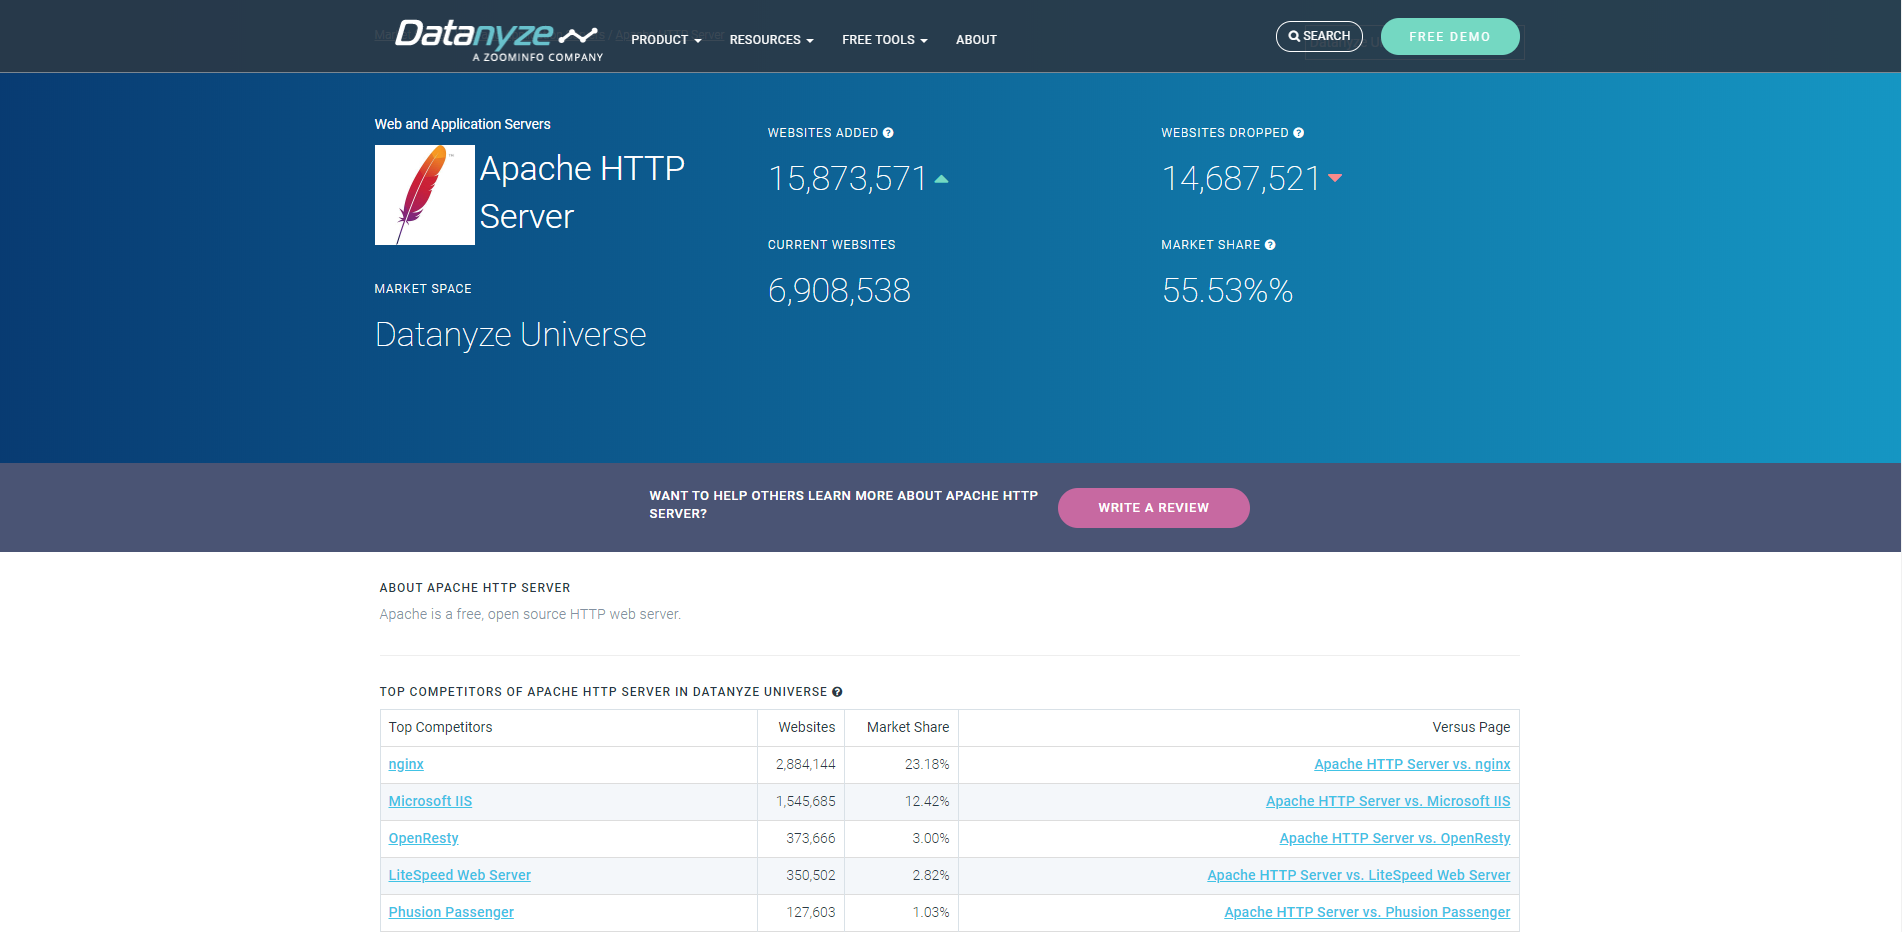
\includegraphics[width=88mm,scale=0.8]{Apdenix/MarketshareApache.PNG}
    \caption{the market share of Apache web servers \cite{Apache}}
    \label{the market share of Apache web servers}
\end{figure}
\subsection*{Learning loop and known IPs} \label{Learning loop and known IP's}

The learning loop described in the MOSCOW shall be fairly basic and the loop will have two primary functions. The first is simply the ability to distinguish malicious IP addresses from the collated data. The secondary function is to identify and flag up potential candidates from the IP collection that could potentially be search engine bots. These requests may have many similarities in architecture. The IP of a bot could have different address patterns, even if sent from the same host, and these bot IPs may change periodically. This would require a larger amount of inputting of data, therefore, it may be easier to have a community driven approach. Due to the potential for abuse such as a hacker adding their IP to the proven bot list, there is a secondary requirement that an overseer approves all the good bots manually.

\subsection*{Database}
For the justification purposes of database type, the different types of database shall be assessed in this section. The first database that has been considered is a NoSQL database namely, MongoDB. MongoDB is a document-oriented database and is currently the most popular NoSQL database at the time of this research.  MongoDB makes it easy to access documents by indexing, hence, it provides a fast query response. A great advantage of MongoDB is that it is a horizontally scalable database, and when you have to handle a large amount of data, it is possible to distribute it to several machines (\cite{MongoDB5}). During the development phase there shall only be one user machine. During the implementation of the software, however, the server will scale, this is an appropriate feature supporting the justification of MongoDB. MongoDB does not support joins in the way a relational database would; it may slow execution and affect performance (\cite{MongoDBComp})) This disadvantage may have a detrimental effect on the operation of the software, as the data will need to be stored on multiple tables. MongoDB stores key names for each value pair. Also, due to 'no functionality of joins', there is a data redundancy trend. This may result in increasing unnecessary usage of memory and once again is a limitation that may effect the software.

Another alternative database type for the software could be an SQL. An advantage of this database is that by using SQL queries, the user can quickly and efficiently retrieve a large number of records from a database. This would have a positive effect on the processing speed while running the software. In the standard SQL, it is very easy to manage the database system. It does not require a substantial amount of code to manage the database system. This will help to keep the code for the database neat and tidy, and the code required for accessing the database will also be kept similarly trim and orderly. SQL can be used in laptops, PCs, servers and even some mobile phones, which will aid in the development of the software through multiple access vectors (\cite{JavaTPoint}). Microsoft access could be used to develop this software as it is a popular SQL database that can easily be run on a computer with Java integration. If this approach is selected as the database candidate, it would also present a key supporting justification for the utilization of java coding, this will be discussed later in the section on the \nameref{Language} for details.  


\subsection*{API }
A lot of the API's may be able to provide data to the software for example, abuse IP's and GOIP's. Free API's are available from many data base hosts that can identify abuse IP's for example (https://www.abuseipdb.com/). This API could be embedded in the software to assist in identifying malicious IP's. An example of an integration technique that is not classified as an API yet still aids in the data provided at the GOIP level is Geolite2. This program helps to locate and pinpoint the coordinates of an incoming IP address hence assists in the identification of malicious IP's. The overall decision to not use API's was made to keep the data that is collected by the software secure. If the choice was made to allow for API's it very well could be the case that an attacker may realise that they have been discovered and this may effect the overall analysis of the software.

\subsection*{Language} \label{Language}
Many languages were considered including Python, C, PHP and Java. Java is architecturally neutral and would work particularly well for the project as it can be run on any machine. As many users will be utilizing the finished software on various platforms, the use of Java would be advantageous. The use of C as a language was also considered. C is a language that runs on many Unix systems on which most servers run, however, in the modern world most website owners do not necessarily have access to the server that their site is hosted on. Another reason for standing against the utilisation of C as a language is that this language may not be appropriate for the development of a user interface that will be required as a vital component of the software. Python was considered as an alternative code for the project, however, the main issue that was discovered with python was its limitations with database access. If compared to popular technologies like JDBC and ODBC, the Python database access layer is found to be somewhat underdeveloped and primitive. Due to the proposed architecture of the software, python would not be a suitable language, as fluid database communication is integral to the project. Finally, PHP was considered as a language for the project because the software could be implemented as a web based application. Unfortunately, this approach may have given the attackers access to the data as it is open sourced. This would defeat the overall objective of the project and the software.  

\subsection*{Data Controller}
The decision was made to limit the influence that the computer has on the mitigation of attacks. Many of the papers mentioned in the literature review applied some kind of machine learning or formulaic protocol to ringfence potential malicious attacks and mitigate them. In the majority of the papers looked at there was a margin of error, or degree of uncertainty with these results due to the methodology in their approach. Due to this, the decision was made to enrol a data assessor to the process in order to filter out the IPs that the software had picked up as potentially malicious. This human approach will allow with 100\% certainty that only malicious IPs will be blocked, reported or otherwise actioned. 